\documentclass[12pt,a4paper]{article}

% --- Pacchetti Fondamentali ---
\usepackage[utf8]{inputenc}         % Codifica input
\usepackage[T1]{fontenc}            % Codifica font
\usepackage[italian]{babel}         % Lingua italiana
\usepackage{geometry}               % Gestione margini
\geometry{a4paper, margin=2.5cm}
\usepackage{graphicx}               % Inserimento immagini
\usepackage{float}
\usepackage{hyperref}               % Link cliccabili
\usepackage{enumitem}               % Liste personalizzate
\usepackage{booktabs}               % Tabelle professionali
\usepackage{eso-pic}                % Per inserire immagini in posizioni assolute
\usepackage{tikz}                   % Disegno vettoriale per il posizionamento
\usepackage{circuitikz}             % Per il disegno di circuiti elettrici
\usepackage{pgfplots}               % Per plottare i diagrammi
\pgfplotsset{compat=1.18}           % Ottimizza la compatibilità e previene avvisi
\usepackage{float}                  % Per l'utilizzo del posizionamento [H] nelle figure
\usepackage{amsmath}                % Per il comando \text nelle formule matematiche
\usepackage{caption}

% --- Pulizia Formattazione Paragrafi ---
\setlength{\parindent}{0pt}         % Elimina l'indentazione automatica ad inizio paragrafo
\setlength{\parskip}{1em}           % Aggiunge spazio verticale tra i paragrafi

% --- Configurazione Hyperref ---
\hypersetup{
    colorlinks=true,
    linkcolor=black,
    filecolor=magenta,      
    urlcolor=cyan,
    pdftitle={Relazione tecnica Sensore - TEII},
}

% --- Inizio Documento ---
\begin{document}

\AddToShipoutPictureBG*{%
  \begin{tikzpicture}[remember picture, overlay]
    \node [anchor=north west, inner sep=30pt] at (current page.north west)
      {
\includegraphics[height=1.5cm]{Misc/diem (1).png}};
  \end{tikzpicture}
}

% ==========================================
% FRONTESPIZIO
% ==========================================
\pagenumbering{Alph} % Evita il conflitto di identificatori di pagina per hyperref

\begin{titlepage}
 
    \centering
    \vspace*{1cm}
    \large \textbf{UNIVERSITÀ DEGLI STUDI DI SALERNO} \\
    \large Corso di Laurea in Ingegneria Informatica \\
    \vspace{0.5cm}
    \rule{\linewidth}{0.2pt} \\
    \vspace{0.5cm}
    \large Corso: \textbf{Tecnologie Elettriche per l'Informatica Industriale} \\
    \large Anno Accademico: \textbf{2025/2026} \\
    
    \vspace{2cm}
    
    \LARGE \textbf{Studio e caratterizzazione di sensori} \\
    \Large \textbf{Circuito analogico per il rilevamento di fiamma: analisi, filtraggio RC e discriminazione dei disturbi non desiderati} \\
    
    \vspace{1.5cm}
    
    \begin{figure}[H]
    \centering
    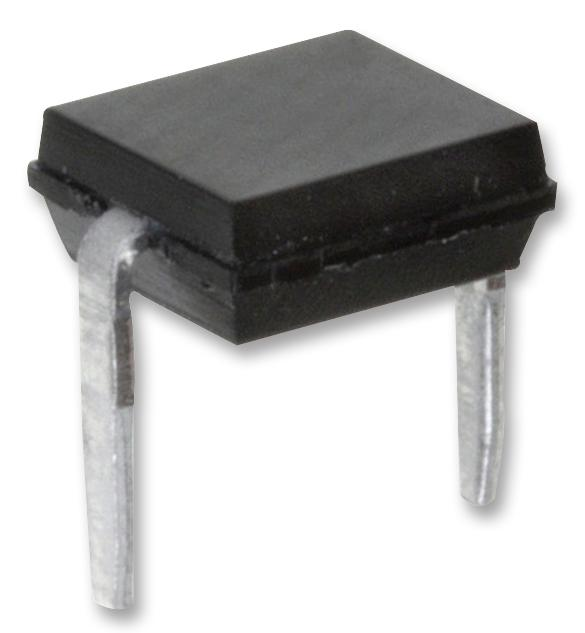
\includegraphics[width=0.2\textwidth]{Misc/bp104.jpg}
	\end{figure}
	
     \vspace{1.5cm}	
    
    \large \textbf{Gruppo: 100} \\
    
    \vspace{2cm}
    
    \begin{table}[h]
        \centering
        \begin{tabular}{lll}
            \textbf{Nome} & \textbf{Cognome} & \textbf{Matricola} \\
            \midrule
            Riccardo  & La Porta & 0612709691 \\
            Lorenzo & Allocco & 0612709084 \\
            Francesco & Grimaldi & 0612708839 \\
            Alessandro & Altieri & 0612709239 \\
        \end{tabular}
    \end{table}

\end{titlepage}

\newpage
\pagenumbering{arabic} % Ripristina la numerazione standard da qui in poi
\tableofcontents
\newpage

% ==========================================
% INTRODUZIONE
% ==========================================
\section{Introduzione}
    Ci siamo posti il problema di avere a disposizione un circuito analogico capace di mettere insieme tutte
    le conoscenze acquisite nel corso. Abbiamo posto attenzione soprattutto alla progettazione di un sistema
    tollerante ai disturbi caratteristici del mondo reale, completamente in accordo con l'obiettivo di proporre
    un'idea sicuramente applicabile nella realtà. Il presente documento presenterà l'analisi, il dimensionamento
    e la progettazione di un circuito integrato analogico per il rilevamento di fiamma a infrarossi, sviluppato
    con l'obiettivo di non essere un semplice dispositivo di rilevamento, ma anche un'architettura di controllo
    analogica completa e autosufficiente. Il sistema, infatti, non si limita a captare lo stimolo luminoso, ma
    elabora il segnale attraverso blocchi sequenziali di condizionamento e isolamento, fino a generare un output
    di commutazione netto e privo di incertezze, pronto per interfacciare e pilotare direttamente uno stadio attuatore
    per l'estinzione dell'incendio.

    L'architettura circuitale proposta si articola in una struttura modulare a blocchi sequenziali,
    ciascuno deputato a una specifica funzione di elaborazione del segnale. Nello specifico, la
    relazione guiderà il lettore attraverso la comprensione dei seguenti stadi hardware:

    \begin{itemize}
        \item \textbf{Stadio di Trasduzione Ottica:} Analisi del fotodiodo, verrà illustrato il principio fisico secondo
            cui la radiazione IR genera una debole fotocorrente e il ruolo della resistenza di carico $R_1$.
        
        \item \textbf{Stadi di Isolamento ad Alta Impedenza (Voltage Follower 1 e 2):} Studio degli amplificatori operazionali
            configurati come inseguitori di tensione con retroazione e la loro natura disaccoppiante.
        
        \item \textbf{Stadio di Filtraggio Passa-Basso:} Dimensionamento di un filtro d'ordine singolo (rete $RC$) dedicato
            all'abbattimento del rumore ad alta frequenza e ai disturbi dovuti al ronzio di rete delle illuminazioni artificiali.
        
        \item \textbf{Stadio di Integrazione Temporale (Debouncer Analogico):} Trattazione del cuore logico del sistema di sicurezza.
            Verrà spiegato matematicamente come il blocco sfrutti la natura dei circuiti RC per ricreare un sistema che inibisce false
            letture. Con questo metodo sarà poi possibile dare al circuito una "tolleranza" rispetto al tempo di esposizione della fiamma
            al fotodiodo.
        
        \item \textbf{Stadio di Commutazione e Output (Comparatore di Soglia):} Descrizione dell'ultimo operazionale operante in anello
            aperto come comparatore di tensione. Verrà analizzato il sistema con cui il circuito riesce a capire quando l'ingresso del
            sistema viene sollecitato effettivamente da una fiamma.
    \end{itemize}

\newpage

\section{Sensore scelto e realtà di interesse}
    Il cuore dello stadio di trasduzione ottica è costituito dal fotodiodo al silicio \textbf{BP104}, un componente con un filtro plastico
    integrato per la luce diurna che, bloccando la radiazione visibile, isola lo spettro \textbf{IR-A} (Infrarosso Vicino). 

    Il principio di funzionamento del componente si basa sull'effetto fotoelettrico interno: quando i fotoni della radiazione IR colpiscono
    la zona di svuotamento della giunzione, trasferiscono la propria energia agli elettroni di valenza, generando coppie elettrone-lacuna.
    Essendo configurato in \textbf{modalità fotoconduttiva} (polarizzazione inversa tramite la tensione $V_{in} = +5\text{ V}$ sul catodo),
    il fotodiodo traduce istantaneamente questo flusso luminoso in una debole fotocorrente inversa ($I_{\text{ph}}$), rigorosamente lineare
    rispetto all'irraggiamento ricevuto (Fig. 3). Tale corrente, scorrendo attraverso la resistenza di carico $R_1$, genera ai suoi capi la
    tensione di ingresso per lo stadio successivo secondo la legge di Ohm:

        \begin{figure}[H]
            \centering
            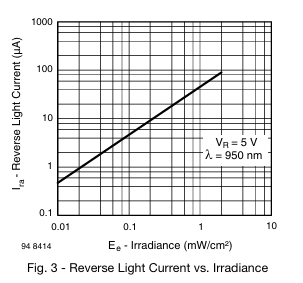
\includegraphics[width=0.5\textwidth]{Misc/corrente_inversa.png}
        \end{figure}
        
        \begin{figure}[H]
            \centering
            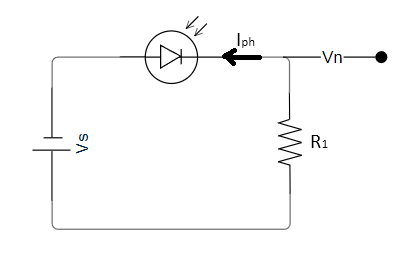
\includegraphics[width=0.5\textwidth]{Misc/pol_diodo.png}
        \end{figure}	
        
    \begin{equation}
        \boxed{V_{\text{n}} = I_{\text{ph}} \cdot R_1}
    \end{equation}

\section{Descrizione preliminare e assunzioni}
    Per procedere con il dimensionamento analitico e la successiva validazione del circuito, è necessario definire lo scenario operativo,
    i parametri elettrici fondamentali e le assunzioni ideali che governano il comportamento dei componenti scelti.

    Il sistema è alimentato da una sorgente in corrente continua ($V_{in}$) stabilizzata a $+5\text{V}$, derivata magari tramite uno stadio
    di regolazione a monte, per garantire un'alimentazione stabile e sicura. Per quanto riguarda i segnali d'ingresso, assumiamo che la
    radiazione emessa da una fiamma libera nello spettro del vicino infrarosso (lunghezza d'onda tipica $\lambda \approx 940\text{ nm}$)
    colpisca la superficie sensibile del fotodiodo inducendo una corrente di conduzione inversa proporzionale all'irraggiamento ottico.

% ==========================================
% PROGETTAZIONE
% ==========================================

\section{Caratteristiche fisiche}

    Come anticipato in precedenza, per la realizzazione del sistema in questione sono stati impiegati vari componenti "non banali", che andremo
    ad analizzare più nel dettaglio nei paragrafi 4.1 e 4.2 sottostanti. Ovviamente ci concentreremo anche nel descrivere il ruolo
    di ogni blocco, il dimensionamento dei componenti e le valutazioni teoriche fatte. Qui sotto è riportato lo schema elettrico dettagliato del
    circuito:

    % Disegno dello schema del diagramma
    \begin{figure}[H]
    \centering
        \begin{circuitikz}[scale=0.75, transform shape]
            
            % ==========================================
            % LINEA DI MASSA COMUNE
            % ==========================================
            % AGGIUNTO "{}" ALLA FINE DI QUESTA LINEA PER RISOLVERE L'ERRORE TIKZ
            \draw (0, 0) node[left] {GND} node[circle, fill, inner sep=1.2pt] {} -- (10.5, 0) node[ground] {} -- (21,0) node[right] {GND} node[circle, fill, inner sep=1.2pt] {};
            
            % ==========================================
            % 1. STADIO: FOTODIODO (Inversa per modalità fotoconduttiva)
            % ==========================================
            \draw (0,3) node[left] {$V_{in}$} node[circle, fill, inner sep=1.2pt] {} -- (1,3)
                    to[photodiode, l_=D, invert] (2.5,3) coordinate (nodoSens);
            \draw (nodoSens) to[R, l_=$R_1$] (2.5,0);
            
            % Scatola tratteggiata Fotodiodo
            \draw[dashed, gray] (0.5,4) rectangle (3.3,0.5);
            \node[text=gray, font=\tiny\bfseries] at (2,4.2) {FOTODIODO};

            % ==========================================
            % 2. STADIO: VOLTAGE FOLLOWER 1 (AMP1)
            % ==========================================
            \draw (5,2.5) node[op amp, yscale=-1] (amp1) {};
            \node[left, font=\tiny, yshift=-0.15cm] at (amp1.-) {};
            \node[left, font=\tiny, yshift=0.15cm] at (amp1.+) {};
            \node[above, font=\small] at (4.9, 2.3) {AMP1};
            \draw (nodoSens) -- (amp1.+);

            % La retroazione si chiude sul meno (-)
            \draw (amp1.out) -- (6.2,2.5) coordinate (nodoVo) {}
                    -- (6.2,1.2) -- (3.8,1.2) -- (amp1.-);
            \node[above, font=\tiny] at (6.1, 2.5) {$V_o$};

            % Disegno un gradino per tornare a y=3
            \draw (nodoVo) -- (6.5, 2.5) -- (6.5, 3) coordinate (nodoLeftR2);

            % Scatola tratteggiata AMP1
            \draw[dashed, gray] (3.6,4) rectangle (6.7,0.5);
            \node[text=gray, font=\tiny\bfseries] at (5.1,4.2) {VOLTAGE FOLLOWER};

            % ==========================================
            % 3. STADIO: FILTRO PASSA-BASSO
            % ==========================================
            \draw (nodoLeftR2) to[R, l_=$R_2$] (9.5,3) coordinate (nodoC1) {};
            \draw (nodoC1) to[C, l_=$C_1$] (9.5,0);
            
            % Scatola tratteggiata Filtro
            \draw[dashed, gray] (7.1,4) rectangle (10.3,0.5);
            \node[text=gray, font=\tiny\bfseries] at (8.7,4.2) {FILTRO PASSA-BASSO};

            % ==========================================
            % 4. STADIO: VOLTAGE FOLLOWER 2 (AMP2)
            % ==========================================
            \draw (12,2.5) node[op amp, yscale=-1] (amp2) {};
            \node[left, font=\tiny, yshift=0.15cm] at (amp2.+) {};
            \node[left, font=\tiny, yshift=-0.15cm] at (amp2.-) {};
            \node[above, font=\small] at (11.9, 2.3) {AMP2};

            % Collegamenti agli ingressi
            \draw (nodoC1) -- (amp2.+);
            \draw (amp2.out) -- (13.2,1.2) -- (10.8,1.2) -- (amp2.-);    
            \node[above, font=\tiny] at (13.1, 2.5) {$V_s$};
            
            % Disegno un gradino per tornare a y=3
            \draw (amp2.out) -- (13.5, 2.5) -- (13.5, 3) coordinate (nodoLeftR3);

            % Scatola tratteggiata AMP2
            \draw[dashed, gray] (10.7,4) rectangle (13.7,0.5);
            \node[text=gray, font=\tiny\bfseries] at (12.2,4.2) {VOLTAGE FOLLOWER};

            % ==========================================
            % 5. STADIO: DEBOUNCER ANALOGICO
            % ==========================================
            \draw (nodoLeftR3) to[R, l_=$R_3$] (16.5,3) coordinate (nodoC2) {};
            \draw (nodoC2) to[C, l_=$C_2$] (16.5,0);
            
            % Scatola tratteggiata Debouncer
            \draw[dashed, gray] (14.1,4) rectangle (17.3,0.5);
            \node[text=gray, font=\tiny\bfseries] at (15.7,4.2) {DEBOUNCER ANALOGICO};

            % ==========================================
            % 6. STADIO: COMPARATORE (AMP3)
            % ==========================================
            \draw (19,2.5) node[op amp, yscale=-1] (amp3) {};
            \node[left, font=\tiny, yshift=0.15cm] at (amp3.+) {};
            \node[left, font=\tiny, yshift=-0.15cm] at (amp3.-) {};
            \node[above, font=\small] at (18.9, 2.3) {AMP3};
            
            % Collegamenti agli ingressi
            \draw (nodoC2) -- (amp3.+); 
            \draw (amp3.-) to[short, -o] (17.8,0.9) node[right, font=\tiny] {$V_{REF}$};
            
            % Uscita
            \draw (amp3.out) -- (20.2, 3) -- (21, 3) node[right] {$V_{out}$} node[circle, fill, inner sep=1.2pt] {};
            
            % Scatola tratteggiata Comparatore
            \draw[dashed, gray] (17.6,4) rectangle (20.4,0.5);
            \node[text=gray, font=\tiny\bfseries] at (19,4.2) {COMPARATORE};

        \end{circuitikz}

        \caption{Schema a blocchi definitivo del sensore di fiamma con debouncer analogico integrato.}
        \label{fig:sensore_fiamma_debouncer}
    \end{figure}

    \subsection{Fotodiodo BP104}
        Il BP104 è un fotodiodo al silicio di tipo PIN ampiamente utilizzato nei sistemi di ricezione a infrarossi. Rispetto
        al più generale BPW34 (che ha una capsula trasparente a spettro totale), il BP104 si distingue per specifiche
        ottiche ed elettriche molto mirate.

        \begin{itemize}
            \item \textbf{Caratteristiche ottiche e spettrali:} La resina epossidica nera che costituisce il case plastico funge da filtro ottico passante e quindi riesce a
                tagliare quasi completamente lo spettro della luce visibile (evitando che la luce del sole o delle lampadine di casa
                falsino la lettura), riuscendo così a essere particolarmente sensibile alla banda IR (È perfettamente accoppiato
                spettralmente con gli emettitori IR all'arseniuro di gallio).

                Scavando nelle caratteristiche più dettagliate del componente in questione , troviamo una banda di sensibilità che
                va da $870\text{ nm}$ a $1050\text{ nm}$ (intervallo in cui la sensibilità non scende sotto il 50\% del picco), con
                un profilo di ricezione decisamente ampio e piatto che va da $+65^\circ$ a $-65^\circ$ circa. A riconferma delle
                ottime caratteristiche tecniche, abbiamo anche un area radiante sensibile di $7.5\text{ mm}^2$, considerata medio
                grande per questa categoria, garantendo un'ottima raccolta di fotoni anche con sorgenti distanti.
            \item \textbf{Caratteristiche elettriche:} Con un'irradiazione $E_e = 1\text{ mW/cm}^2$ a $\lambda = 950\text{ nm}$ e una tensione inversa $V_R = 5\text{ V}$,
                riusciamo ad ottenere una corrente di luce inversa ($I_{ra}$) di circa $40 - 45\,\mu\text{A}$. Rifacendoci invece a
                dei parametri più assoluti troviamo anche una corrente di buio inversa ($I_{r0}$) tipicamente tra $2\text{ nA}$ e
                $30\text{ nA}$, una tensione di breakdown inverso ($V_{(BR)}$) minima di $60\text{ V}$, una tensione a circuito
                aperto ($V_o$) di $350\text{ mV}$ e una corrente di cortocircuito ($I_k$) di $38\,\mu\text{A}$.
            \item \textbf{Limiti massimi e caratteristiche termo-meccaniche:} Con una dissipazione di potenza massima di 215 mW, una
                temperatura operativa nel range da $-40^\circ\text{C}$ a $+100^\circ\text{C}$ e anche un package plastico di tipo Trough-Hole
                orientato alla ricezione dall'alto troviamo un vantaggio meccanico e chimico dal punto di vista della sensibilità dell'
                ambiente circostante da parte del fotodiodo che ci permette di determinare in modo abbastanza accurato le condizioni
                che dobbiamo garantirgli per permettere un lavoro notevolmente accurato.
        \end{itemize}

    \subsection{Amplificatore Operazionale TL082}
        Il TL082 è un amplificatore operazionale doppio ad alta velocità che integra, in un unico package plastico a 8 pin, due circuiti operazionali 
        indipendenti. Rispetto ai dispositivi più datati a transistor bipolari (come lo storico $\mu$A741), il TL082 si distingue per l'utilizzo di 
        transistori a effetto di campo a giunzione (\textbf{JFET}) nello stadio di ingresso, una scelta tecnologica che offre specifiche elettriche e 
        dinamiche decisamente mirate per il condizionamento dei segnali.

        \begin{itemize}
            \item \textbf{Caratteristiche d'ingresso ad alta impedenza:} L'impiego dei JFET nella sezione d'ingresso permette al componente di esibire 
                un'impedenza d'ingresso straordinariamente elevata, tipicamente pari a $10^{12}\,\Omega$ ($1\text{ T}\Omega$). Questa specifica è di 
                fondamentale importanza nel nostro circuito, poiché garantisce che gli stadi \texttt{AMP1} e \texttt{AMP2} possano interfacciarsi con 
                le alte resistenze dei blocchi passivi (quali $R_1 = 1\text{ M}\Omega$) senza assorbire correnti significative. 

                A riconferma di ciò, la corrente di polarizzazione d'ingresso (\textit{input bias current}) si attesta su livelli microscopici, con un 
                valore tipico di appena $30\text{ pA}$ a temperatura ambiente. Questo previene qualsiasi sensibile caduta di tensione parassita ai capi 
                delle resistenze di condizionamento, azzerando gli errori di offset sistematici che avrebbero altrimenti inficiato l'accuratezza del sensore.
            
            \item \textbf{Caratteristiche elettriche e dinamiche di frequenza:} Alimentato in regime singolo a $+5\text{V}$, l'operazionale esprime un elevato 
                guadagno di tensione ad anello aperto (\textit{open-loop voltage gain}), pari a circa $200\text{ V/mV}$ ($106\text{ dB}$). Dal punto di vista
                della risposta dinamica, il TL082 presenta uno \textit{Slew Rate} tipico molto elevato, pari a $13\text{ V}/\mu\text{s}$, assistito da una banda 
                passante a guadagno unitario (\textit{gain-bandwidth product}) di $4\text{ MHz}$. 
            
                Questi parametri dinamici assicurano una velocità di risposta eccellente e tempi di assestamento ridotti, traducendosi in una commutazione d'uscita 
                estremamente netta e priva di oscillazioni spurie nel momento in cui il terzo stadio (\texttt{AMP3}) opera in anello aperto come comparatore di soglia.
            
            \item \textbf{Limiti massimi e caratteristiche termo-meccaniche:} Il componente garantisce una temperatura operativa di lavoro standard compresa nel range 
                tra $0^\circ\text{C}$ e $+70^\circ\text{C}$ (per la serie commerciale standard), con una capacità di dissipazione di potenza massima continua di circa $680\text{ mW}$. 
            
                Il package plastico di tipo \textit{Dual In-line Package} (DIP-8) a saldatura passante offre una notevole robustezza meccanica e una disposizione simmetrica dei 
                pin che semplifica l'ingegnerizzazione del circuito stampato, permettendo di alimentare e configurare entrambi i buffer di isolamento del sistema riducendo l'ingombro 
                spaziale complessivo sulla scheda.
        \end{itemize}
    
    \subsection{1$^\circ$ STADIO - Fotodiodo con convertitore di tensione}
        Questo stadio si occupa di acquisire il segnale luminoso nella banda dell'infrarosso vicino (IR-A) rilevato dal fotodiodo
        (\texttt{D}) nell'ambiente circostante, tenendo in considerazione che in questa fase l'informazione è ancora fortemente influenzata
        dai disturbi ad alta frequenza e dalle fluttuazioni ottiche non desiderate.

        Il fotodiodo BP104, per via dell'\textbf{effetto fotoelettrico interno}, genera una corrente di conduzione inversa (fotocorrente)
        proporzionale all'irraggiamento ottico ricevuto. Questa corrente, essendo nell'ordine dei micro-ampere ($\mu\text{A}$), deve essere
        necessariamente convertita in una tensione elettrica prima di poter essere elaborata dai blocchi successivi. Il disaccoppiatore di 
        rete posto subito dopo (\texttt{AMP1}), infatti, presenta un'impedenza d'ingresso ideale e richiede una grandezza in tensione per poter
        operare correttamente.

        Per realizzare questa conversione d'interfaccia, si inserisce un resistore ($R_1$) in serie al fotodiodo, collegato direttamente verso 
        la massa comune (GND), sfruttando la caduta di potenziale che si sviluppa ai suoi capi per effetto della legge di Ohm. Poiché la fotocorrente 
        generata dal sensore è intrinsecamente molto esigua, è fondamentale adottare un valore di resistenza estremamente elevato per ottenere un segnale 
        in tensione con una dinamica apprezzabile e facilmente rilevabile. Per questo motivo si è optato per una resistenza di conversione pari a 
        $1\text{ M}\Omega$, la quale garantisce un'escursione termica del segnale di diversi volt anche a fronte di deboli irraggiamenti causati da fiamme distanti.
        
    \newpage

    \subsection{2$^\circ$ e 4$^\circ$ STADIO - Disaccoppiatore di rete}
        Gli stadi di trasduzione (1), filtraggio (3) e integrazione/decisione (5-6) richiedono un dimensionamento
        indipendente per preservare le rispettive risposte in frequenza e costanti di tempo. Affinché la loro
        interconnessione in cascata non alteri le funzioni di trasferimento locali, è indispensabile introdurre un
        meccanismo di isolamento, tecnicamente definito \textbf{disaccoppiamento d'impedenza}. 

        Nelle catene analogiche, l'accoppiamento ideale si realizza interponendo uno stadio che presenti un'impedenza
        d'ingresso tendente al circuito aperto (valore teoricamente infinito) e un'impedenza d'uscita tendente al cortocircuito
        (valore teoricamente nullo). La topologia ottimale per adempiere a questa funzione è l'amplificatore operazionale in
        configurazione \textbf{voltage follower} (o inseguitore di tensione, implementato nei blocchi \texttt{AMP1} e \texttt{AMP2}).
        Questa struttura replica fedelmente sul terminale d'uscita la tensione applicata all'ingresso (guadagno unitario, $A_v = 1$),
        garantendo al contempo le proprietà impedenziali necessarie a eliminare l'effetto di carico tra i moduli passivi.

    \subsection{3$^\circ$ STADIO - Filtro Passa-Basso}
        Questo stadio è posto in cascata all'ingresso unicamente per filtrare tutto il rumore in alta frequenza che non ci interessa.
        Ovviamente questa assunzione si può fare nel momento in cui, dopo aver analizzato lo spettro dinamico di una fiamma, ci rendiamo
        conto che lo sfarfallio (\textit{flickering}) macroscopico della stessa introduce una modulazione del segnale elettrico a bassissima
        frequenza (stimata tra 1 e 2 Hz) e a questo punto allora possiamo concludere che lo stadio di filtraggio dovrà prevedere un filtro
        passa-basso con una banda passante che si aggiri intorno alla frequenza individuata precedentemente.

        Per realizzare questo stadio abbiamo bisogno di un resistore ($R_2$) e di un condensatore ($C_1$) da dimensionare opportunamente.
        Tenendo conto che la frequenza di taglio di un filtro passa-basso si trova come:

        \begin{equation}
            \boxed{f_T = \frac{1}{2\pi RC}}
        \end{equation}

        e che la resistenza deve essere dimensionata opportunamente per non limitare o aumentare troppo la corrente passante in questo stadio
        (un buon valore di compromesso è stato individuato intorno ai 3 k$\Omega$), bisogna trovare una dimensione di capacità del condensatore
        che ci permetta di poter trovare una $f_T$ che si aggira al di sotto dei 3-4 Hz. E' stata scelta la capacità commerciale di 22 $\mu$F che ci dà quindi
        una $f_T \approx 2.41 Hz$, perfettamente in accordo con il valore ricercato.

        \begin{figure}[H]
        \centering
        \begin{tikzpicture}
            \begin{axis}[
                width=11cm, height=6.5cm,   % Leggermente più alto visto che è singolo
                xmode=log,                  % Asse X logaritmico
                xmin=0.01, xmax=1000,         % Range frequenze da 1 Hz a 10 kHz
                xlabel={Frequenza [Hz]},
                ylabel={Magnitudo [dB]},
                ymin=-40, ymax=5,
                ytick={-30, -20, -10, -3, 0}, % Tick a -3 dB per la frequenza di taglio
                grid=both,
                minor grid style={dashed, gray!30},
                major grid style={gray!60},
                tick label style={font=\footnotesize},
                label style={font=\small}
            ]
            
            % Funzione analitica del solo filtro passa-basso: 1 / sqrt(1 + (2*pi*x*tau)^2)
            \addplot[red, thick, domain=0.01:1000, samples=200] 
                {20*log10( 1 / sqrt(1 + (2*pi*x*0.066)^2) )};
                
            \end{axis}
        \end{tikzpicture}
        
        % PROPRIETÀ INLINE: Applica la formattazione solo a questa caption
        \captionsetup{justification=centering, singlelinecheck=false, font=small}
        \caption{Diagramma di Bode (Modulo) del filtro passa-basso}
        \label{fig:bode_passabasso_modulo}
        \end{figure}
    
    \subsection{5$^\circ$ STADIO - Debouncer analogico}
        Il quinto blocco funzionale costituisce l'elemento centrale per la sicurezza e l'immunità ai falsi allarmi dell'intera architettura analogica. 
        Denominato 'Debouncer Analogico', questo stadio ha il compito di discriminare gli impulsi luminosi intensi ma transitori (quali il flash di una 
        fotocamera, variazioni repentine dell'illuminazione ambientale o riflessi solari momentanei) da un incendio effettivo, il quale presenta una 
        persistenza temporale macroscopica.

        La topologia circuitale è basata su una rete passiva integratrice $R_3 - C_2$, interposta tra l'uscita a bassa impedenza del secondo buffer 
        (\texttt{AMP2}) e l'ingresso ad alta impedenza del comparatore finale (\texttt{AMP3}). Grazie al perfetto disaccoppiamento d'impedenza garantito 
        dagli operazionali a monte e a valle, il comportamento dinamico di questo stadio è isolato e governato esclusivamente dai valori dei suoi due componenti passivi.

        Quando il fotodiodo rileva una sorgente IR stabile e il segnale supera il filtraggio iniziale, l'uscita di \texttt{AMP2} si porta repentinamente 
        al valore di regime alto, che approssimiamo alla tensione di alimentazione del sistema ($V_s \approx V_{max} = +5\text{ V}$). Il condensatore $C_2$, 
        inizialmente scarico, non asseconda istantaneamente il gradino di tensione ma comincia ad accumulare carica elettrica attraverso il resistore $R_3$. 
        La transizione della tensione ai capi del condensatore ($V_{C2}$) nel dominio del tempo risponde alla legge esponenziale costitutiva dei circuiti $RC$:

        \begin{equation}
            V_{C2}(t) = V_{max} \cdot \left(1 - e^{-\frac{t}{\tau_2}}\right)
        \end{equation}

        dove $\tau_2 = R_3 \cdot C_2$ rappresenta la costante di tempo intrinseca del debouncer. Per adempiere alla funzione di anti-falso allarme, questa costante 
        viene dimensionata in modo da essere significativamente più grande rispetto alla costante $\tau_1$ del filtro passa-basso precedente. Nel nostro caso, 
        avendo selezionato i valori commerciali di $R_3 = 10\text{ k}\Omega$ e $C_2 = 100\,\mu\text{F}$, la costante di tempo risulta:

        \begin{equation}
            \tau_2 = 10.000\,\Omega \cdot 100 \cdot 10^{-6}\text{ F} = 1\text{ s}
        \end{equation}

        L'efficacia di questa scelta progettuale si traduce direttamente in una protezione bidirezionale del sistema:
        
        \begin{itemize}
            \item \textbf{Comportamento ai transitori veloci (Disturbi):} Se la sorgente IR subisce un'attivazione impulsiva (durata $\Delta t \ll \tau_2$), la tensione 
                $V_{C2}(t)$ sale solo di una piccola frazione di volt. Non appena l'impulso cessa, il condensatore si scarica rapidamente attraverso $R_3$ verso l'uscita 
                di \texttt{AMP2} (che nel frattempo è tornata a $0\text{V}$), impedendo alla tensione di raggiungere la soglia di scatto del comparatore.
            \item \textbf{Comportamento a segnali persistenti (Incendio reale):} Se l'esposizione della fiamma sul fotodiodo è continua e stabile ($t > \tau_2$), la curva 
                esponenziale ha il tempo necessario per salire oltre il valore di riferimento $V_{REF}$ impostato sullo stadio successivo, validando l'allarme e abilitando 
                la commutazione dell'output.
        \end{itemize}

        In sintesi, lo stadio agisce come un decisore a memoria analogica: accumula l'energia del segnale ottico nel tempo e "accetta" lo stimolo come un incendio reale 
        solo se quest'ultimo dimostra una persistenza fisica coerente con il fenomeno macroscopico di una combustione.

    \subsection{6$^\circ$ STADIO - Comparatore di Soglia e Output}
        Il sesto stadio del circuito di condizionamento è deputato alla conversione del segnale analogico integrato in un segnale digitale binario ($0\text{V}$ o $+5\text{V}$), 
        idoneo a pilotare in totale sicurezza lo stadio attuatore a valle. Questa funzione di decisione logica viene assolta dall'ultimo amplificatore operazionale (\texttt{AMP3}), 
        configurato come \textbf{comparatore di soglia in anello aperto} (open-loop).

        Grazie alla configurazione ad anello aperto, l'operazionale non presenta alcuna rete di retroazione tra l'uscita e gli ingressi. Di conseguenza, il componente esprime il suo
        massimo guadagno differenziale ($A_{ol} \to \infty$). Una minima differenza di potenziale tra i suoi due terminali d'ingresso porta istantaneamente l'uscita in saturazione 
        positiva o negativa, azzerando le zone di incertezza elettrica.

        Il terminale non-invertente ($+$) di \texttt{AMP3} è collegato direttamente al nodo del debouncer analogico, ricevendone la tensione esponenziale $V_{C2}(t)$. Il terminale invertente
        ($-$) è invece vincolato a una tensione di riferimento costante $V_{REF}$ (impostabile fisicamente tramite un partitore resistivo o un potenziometro di precisione). Il comportamento 
        dell'uscita finale $V_{out}$ risponde rigorosamente alla seguente legge matematica:
        
        \begin{equation}
            V_{out} = 
            \begin{cases} 
            V_{OH} \approx +5\text{V} & \text{se } V_{C2}(t) > V_{REF} \quad \text{(Allarme: Fiamma validata)} \\ 
            V_{OL} \approx 0\text{V} & \text{se } V_{C2}(t) < V_{REF} \quad \text{(Sicurezza: Riposo o disturbo isolato)} 
            \end{cases}
        \end{equation}

        L'interazione analitica tra lo stadio integratore (Debouncer) e il comparatore permette di calcolare esattamente il tempo minimo di esposizione continua alla fiamma ($t_{min}$)
        necessario a far scattare il sistema di sicurezza. Sostituendo la legge di carica del condensatore nella condizione di scatto $V_{C2}(t) = V_{REF}$, si ottiene:

        \begin{equation}
            V_{REF} = V_{max} \cdot \left(1 - e^{-\frac{t_{min}}{R_3 C_2}}\right)
        \end{equation}

        Esplicitando l'equazione rispetto alla variabile temporale $t_{min}$ tramite l'applicazione delle proprietà dei logaritmi naturali, si ricava la relazione fondamentale di dimensionamento:
        
        \begin{equation}
            \boxed{t_{min} = -R_3 C_2 \cdot \ln\left(1 - \frac{V_{REF}}{V_{max}}\right)}
        \end{equation}

        Questa formula evidenzia l'estrema versatilità del circuito: mantenendo fissi i componenti passivi del debouncer ($R_3 = 10\text{ k}\Omega$ e $C_2 = 100\,\mu\text{F}$, da cui $\tau_2 = 1\text{ s}$), 
        è possibile tarare il tempo di reazione del sistema semplicemente calibrando la tensione di soglia $V_{REF}$. Ad esempio, impostando una $V_{REF} = 3.16\text{ V}$ (pari a circa il $63.2\%$ di 
        $V_{max} = 5\text{V}$), il logaritmo assume valore unitario e il tempo di esposizione richiesto coinciderà esattamente con la costante di tempo dello stadio precedente ($t_{min} = \tau_2 = 1\text{ s}$). 

        La commutazione netta così ottenuta garantisce che l'attuatore finale riceva un comando privo di ambiguità, salvaguardando i dispositivi di potenza da stati di parziale conduzione lineare.

    \subsection{Attuatore - Interfaccia di potenza e logica di accoppiamento}
        L'uscita del comparatore di soglia (\texttt{AMP3}) fornisce un segnale logico binario ben definito: assume il valore di massa ($0\text{V}$) in condizioni 
        di riposo e il valore massimo di alimentazione ($V_{max}$) in caso di allarme validato. Tuttavia, questo segnale possiede soltanto un'informazione di tipo 
        logico-informativo e non l'energia fisica necessaria a compiere un lavoro meccanico o idraulico. Gli amplificatori operazionali, infatti, sono strutturalmente 
        progettati per elaborare segnali e non per erogare correnti elevate; se si tentasse di collegare direttamente l'uscita del comparatore a un carico reale (un attuatore), 
        l'operazionale subirebbe un drastico crollo della tensione d'uscita o un danneggiamento permanente per sovracorrente.

        Per superare questo limite ingegneristico e rendere il sistema autosufficiente, si rende necessaria l'integrazione di uno stadio finale denominato \textbf{Interfaccia di Potenza} 
        (o \textit{Driver} di potenza), il cui compito è separare nettamente la logica di controllo a bassa corrente dal circuito di attuazione ad alta corrente.

        \subsubsection{Il principio dell'Interruttore Elettronico Controllato}
            Il metodo più efficiente e lineare per realizzare questa trasformazione consiste nell'utilizzare un \textbf{transistore di potenza} operante in regime di commutazione 
            (ovvero come interruttore statico). Questo dispositivo può essere immaginato idealmente come un interruttore a tre terminali:
            
            \begin{itemize}
                \item \textbf{Terminale di Controllo (Ingresso):} Connesso all'uscita $V_{out}$ del comparatore, pilota l'apertura o la chiusura del canale assorbendo una corrente praticamente nulla.
                \item \textbf{Terminale di Potenza (Uscita):} Collegato in serie al carico d'interesse.
                \item \textbf{Terminale di Riferimento:} Vincolato alla massa comune (\texttt{GND}) del sistema.
            \end{itemize}

            Il vantaggio fondamentale di questa configurazione risiede nella capacità del terminale di controllo di governare il passaggio di flussi di corrente molto elevati nel circuito di uscita, 
            attingendo l'energia da una linea di alimentazione ausiliaria dedicata, senza gravare sulla sensibile elettronica di condizionamento a monte.

        \subsubsection{Logica di funzionamento e stati di commutazione}
            Una volta interposta questa interfaccia, l'attivazione dell'attuatore risponde a due precisi regimi fisici:
            
            \begin{itemize}
                \item \textbf{Stato di Interdizione (Condizione di Riposo):} Quando il circuito non rileva emergenze, il comparatore mantiene $V_{out} = 0\text{V}$. Il terminale di controllo del transistore 
                    non riceve alcuna sollecitazione energetica. L'interruttore elettronico rimane conseguentemente \textbf{aperto}. In questo stato, il circuito di potenza è interrotto, la corrente non può 
                    scorrere e l'attuatore rimane spento e in totale sicurezza.
                \item \textbf{Stato di Conduzione (Condizione di Allarme):} Al superamento del tempo minimo di esposizione della fiamma sul fotodiodo, $V_{out}$ commuta bruscamente al livello alto ($V_{max}$). 
                    Questa tensione eccita il terminale di controllo del transistore, forzando l'interruttore elettronico a \textbf{chiudersi} istantaneamente verso massa. Il circuito di potenza si completa: 
                    la corrente proveniente dalla sorgente ausiliaria attraversa interamente l'attuatore, attivando immediatamente i sistemi fisici di spegnimento o evacuazione.
            \end{itemize}

        \subsubsection{Protezione dai transitori induttivi di ritorno}
            Molti degli attuatori impiegati nei sistemi antincendio reali (quali bobine di elettrovalvole, relè o teleruttori) sono componenti intrinsecamente induttivi. Per le leggi dell'elettromagnetismo, 
            un'induttanza accumula energia sotto forma di campo magnetico durante la fase di conduzione. 

            Nel momento esatto in cui l'allarme cessa e l'interruttore elettronico si riapre bruscamente per disattivare l'impianto, l'interruzione repentina della corrente genera una forza elettromotrice 
            inversa macroscopica ($V = L \cdot \frac{di}{dt}$). Questo fenomeno si traduce in una violenta sovratensione riflessa, capace di perforare le giunzioni del transistore e distruggerlo. Per garantire 
            l'affidabilità a lungo termine dell'architettura, viene inserito un \textbf{elemento di ricircolo unidirezionale} (un diodo di protezione) in parallelo all'attuatore. Questo componente offre una via 
            di fuga preferenziale e sicura all'energia magnetica residua, smorzando la sovratensione e preservando l'integrità strutturale dell'interfaccia di potenza.

    \subsection{Ambiti di applicazione e scenari operativi}
        L'architettura analogica modulare analizzata si colloca come soluzione ideale in tutti quegli scenari di sicurezza civile e industriale in cui i sistemi di rilevamento convenzionali (quali i sensori di fumo 
        ottici a ionizzazione o i rilevatori termici) risultano intrinsecamente inefficienti, tardivi nella risposta o soggetti a continui falsi allarmi a causa delle normali attività ambientali. 

        Il vantaggio competitivo di un'architettura basata sul monitoraggio della radiazione infrarossa vicina (IR-A), assistita da un filtro ottico per la luce diurna e da uno stadio di integrazione temporale 
        (debouncer), si esprime prevalentemente nei seguenti contesti stazionari:

        \begin{itemize}
            \item \textbf{Autorimesse e parcheggi sotterranei:} In questi ambienti, la presenza costante di gas di scarico, polveri sottili e vapori genererebbe sistematiche attivazioni improprie nei comuni rilevatori 
                di fumo. Al contrario, il sistema analogico proposto ignora la presenza di aerosol e corpi particolati in sospensione, reagendo esclusivamente alla firma radiante termica di una combustione attiva.
            \item \textbf{Locali caldaie e centrali termiche industriali:} Ambienti caratterizzati da repentine variazioni termiche macroscopiche mettono in crisi i sensori di temperatura (termovelocimetrici). Il sensore 
                ottico, operando alla velocità della luce nella banda IR, garantisce un tempo di intervento quasi istantaneo all'insorgere del focolaio, permettendo l'isolamento immediato delle condotte di combustibile 
                prima che l'incendio si propaghi.
            \item \textbf{Aree ad alto affollamento e illuminazione eterogenea:} In strutture quali centri commerciali, teatri o complessi industriali, la presenza di illuminazioni artificiali fluorescenti, LED o a scarica 
                introduce un forte rumore di fondo a frequenza di rete ($50\text{ Hz}$ / $100\text{ Hz}$). Grazie alla combinazione del filtro passa-basso (che abbatte i disturbi in frequenza) e del debouncer analogico 
                (che assorbe i transitori luminosi veloci o i riflessi casuali), l'architettura garantisce una continuità di servizio esente da falsi allarmi.
        \end{itemize}

% ==========================================
% CONCLUSIONI E SVILUPPI FUTURI
% ==========================================

\section{Conclusioni e sviluppi futuri}
    Il lavoro di analisi e progettazione documentato nella presente relazione ha permesso di caratterizzare con successo un'architettura circuitale interamente analogica, dedicata al rilevamento sicuro e tempestivo di fiamme 
    libere tramite la banda spettrale dell'infrarosso vicino (IR-A). L'intero percorso metodologico ha evidenziato come l'adozione di un approccio modulare a blocchi sequenziali sia la chiave ingegneristica per risolvere problemi 
    complessi di condizionamento del segnale, trasformando una microscopica fotocorrente parassita in un robusto segnale di potenza capace di governare un attuatore meccanico di evacuazione o estinzione.

    A valle di tutto ciò, l'architettura presenta comunque degli accorgimenti da poter adottare:

    \begin{enumerate}
        \item \textbf{Integrazione a doppia tecnologia (IR / UV):} Per massimizzare l'immunità ai disturbi, il sistema potrebbe essere espanso integrando un secondo canale di trasduzione ottica parallelo, basato su un sensore sensibile alla 
            radiazione ultravioletta (UV). Convogliando i due output logici a un blocco di commutazione a coincidenza analogica (porta logica AND analogica), l'allarme finale verrebbe abilitato solo se la sorgente emettesse contemporaneamente 
            nello spettro IR e UV, azzerando la probabilità di falsi allarmi anche negli ambienti industriali più ostili.
        \item \textbf{Implementazione di un circuito di scarica rapida asimmetrico:} Attualmente, il debouncer analogico presenta lo stesso tempo sia in fase di carica (attivazione dell'allarme) sia in fase di scarica (cessazione dell'allarme). 
            Inserendo un diodo di bypass in parallelo alla resistenza $R_3$, si potrebbe ottenere un sistema asimmetrico: un tempo di attivazione controllato e lento (es. $1\text{ s}$) associato a uno spegnimento dell'allarme e del sistema di 
            estinzione pressoché istantaneo non appena la fiamma scompare dal campo visivo del fotodiodo.
    \end{enumerate}

\end{document}